%% ============================================================
%% Master's Thesis Defense — Nidanur Günay
%% Abstraction Mechanisms for Virtual Avatars
%% 20 minutes. Weighted towards Evaluation, Discussion,
%% Limitations and Conclusion. Front chapters are a skeleton.
%% Compile from the PROJECT ROOT:
%%   pdflatex -interaction=nonstopmode Defense_Slides.tex
%% ============================================================

\documentclass[aspectratio=169,10pt]{beamer}

\usetheme{default}
\usepackage[T1]{fontenc}
\usepackage[utf8]{inputenc}
\usepackage{helvet}
\renewcommand{\familydefault}{\sfdefault}
\usepackage{graphicx}
\usepackage{booktabs}
\usepackage{tabularx}
\usepackage{xcolor}
\usepackage{tikz}
\usetikzlibrary{positioning, arrows.meta, shapes.geometric}

\graphicspath{{thesis/figures/}{thesis/figures/user_study/}{thesis/}}

%% ---- Colours ----
\definecolor{knblue}{HTML}{00539F}
\definecolor{knlight}{HTML}{E8F0F8}
\definecolor{knaccent}{HTML}{D97706}
\definecolor{knred}{HTML}{B3261E}
\definecolor{kngreen}{HTML}{1B7A43}
\definecolor{kngrey}{HTML}{5A6570}

%% ---- Beamer look ----
\setbeamercolor{structure}{fg=knblue}
\setbeamercolor{frametitle}{fg=knblue}
\setbeamercolor{title}{fg=knblue}
\setbeamerfont{frametitle}{size=\large,series=\bfseries}
\setbeamerfont{title}{size=\LARGE,series=\bfseries}
\setbeamertemplate{navigation symbols}{}
\setbeamertemplate{itemize items}[circle]
\setbeamercolor{itemize item}{fg=knblue}
\setbeamercolor{itemize subitem}{fg=kngrey}
\setbeamerfont{itemize/enumerate subbody}{size=\small}

\makeatletter
\setbeamertemplate{frametitle}{%
  \vspace{0.35em}%
  \hspace{0.3em}\usebeamerfont{frametitle}\usebeamercolor[fg]{frametitle}\insertframetitle%
  \ifx\insertframesubtitle\@empty\else
    \\[0.15em]\hspace{0.3em}{\small\normalfont\color{kngrey}\insertframesubtitle}%
  \fi
  \\[0.25em]\hspace{0.3em}{\color{knblue}\rule{0.965\paperwidth}{1pt}}%
}
\makeatother

\setbeamertemplate{footline}{%
  \hspace{0.9em}{\tiny\color{kngrey}Nidanur Günay\quad|\quad Abstraction Mechanisms for Virtual Avatars}%
  \hfill{\tiny\color{kngrey}\insertframenumber}\hspace{0.9em}\vspace{0.5em}%
}

%% ---- Small helpers ----
\newcommand{\hl}[1]{{\color{knblue}\textbf{#1}}}
\newcommand{\good}[1]{{\color{kngreen}\textbf{#1}}}
\newcommand{\bad}[1]{{\color{knred}\textbf{#1}}}
\newcommand{\sn}[1]{{\color{kngrey}\small #1}}

% Verdict badge
\newcommand{\verdict}[2]{%
  \tikz[baseline=(x.base)]{\node[fill=#1,text=white,rounded corners=2pt,inner xsep=5pt,inner ysep=2pt,font=\footnotesize\bfseries] (x) {#2};}}

% Takeaway strip at the bottom of a slide
\newcommand{\takeaway}[1]{%
  \vfill
  \noindent\colorbox{knlight}{\parbox{0.975\textwidth}{\small\color{knblue}\textbf{Takeaway.} #1}}%
  \vspace{0.2em}}

\title{Abstraction Mechanisms for Virtual Avatars}
\subtitle{Non-Photorealistic Rendering across Avatar Platforms and its Effect on Perceived Trust}
\author{Nidanur Günay}
\institute{Department of Computer and Information Science\\University of Konstanz}
\date{Master's Thesis Defense \quad|\quad 2026}

\begin{document}

%% ============================================================
%% 1 — Title
%% ============================================================
\begin{frame}[plain]
  \vspace{0.5em}
  \begin{center}
    
\includegraphics[width=0.24\textwidth]{UniKonstanz_Logo_Minimum_sRGB}\\[1.2em]
    {\LARGE\bfseries\color{knblue} Abstraction Mechanisms for Virtual Avatars}\\[0.5em]
    {\small\color{kngrey} Non-Photorealistic Rendering across Avatar Platforms\\ and its Effect on Perceived Trust}\\[1.6em]
    {\large Nidanur Günay}\\[0.4em]
    {\footnotesize\color{kngrey} Master's Thesis Defense}\\[1.2em]
    {\footnotesize First reviewer: Prof.\ Dr.\ Oliver Deussen}\\
    {\footnotesize Second reviewer: Prof.\ Dr.\ Tiare Feuchtner}\\[0.8em]
    {\footnotesize\color{kngrey} University of Konstanz, 2026}
  \end{center}
\end{frame}

%% ============================================================
%% PART 0 — SKELETON: problem, questions, what was built
%% ============================================================

\begin{frame}{The problem}{Realism does not buy trust}
  \begin{columns}[T]
    \begin{column}{0.56\textwidth}
      \begin{itemize}
        \item Virtual humans now advise, teach and sell. How they look changes how much people believe them.
        \item Human likeness raises trust, \hl{but not linearly}. Almost-human characters fall into the \hl{uncanny valley}.
        \item \hl{Non-Photorealistic Rendering (NPR)} moves an avatar back down the realism axis on purpose.
      \end{itemize}
      \vspace{0.5em}
      \colorbox{knlight}{\parbox{0.95\textwidth}{\small\color{knblue}
      \textbf{1.} Avatar platforms expose very unequal rendering access.\\[0.25em]
      \textbf{2.} Nobody has measured what the abstraction does to trust.}}
    \end{column}
    \begin{column}{0.42\textwidth}
      \vspace{0.4em}
      \centering
      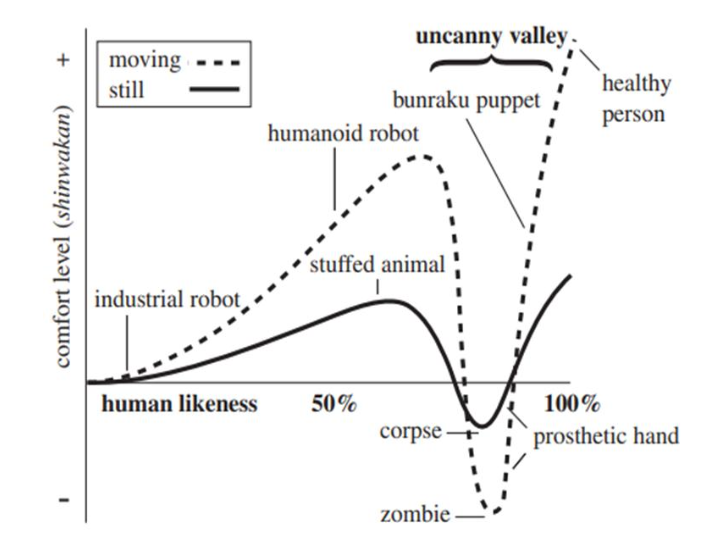
\includegraphics[width=\textwidth]{uncanny_valley_mori}\\[0.3em]
      \sn{The uncanny valley (Mori, 1970)}
    \end{column}
  \end{columns}
\end{frame}

\begin{frame}{Research questions}
  \vspace{0.8em}
  \begin{block}{\textbf{RQ1} \quad Technical transfer}
    How can NPR techniques be adapted to avatar platforms with different rendering architectures, and what does each platform allow or forbid?
  \end{block}
  \vspace{0.3em}
  \begin{block}{\textbf{RQ2} \quad Technique selection}
    Which technique or combination best balances visual abstraction against facial legibility?
  \end{block}
  \vspace{0.3em}
  \begin{block}{\textbf{RQ3} \quad Perception}
    How does NPR stylisation affect perceived eeriness and trustworthiness, and can a stylised avatar reach a photorealistic avatar and a real human speaker?
  \end{block}
  \vspace{0.5em}
  \sn{RQ1 and RQ2 are answered by the system. RQ3 is answered by the user study, which is where this talk spends most of its time.}
\end{frame}

\begin{frame}{What was built}{Eight techniques, three platforms, one shader system}
  \vspace{0.2em}
  \begin{columns}[T]
    \begin{column}{0.60\textwidth}
      \small
      \begin{tabular}{@{}ll@{}}
        \toprule
        \textbf{Version} & \textbf{Limitation it answers} \\
        \midrule
        V1 \enspace Silhouette outline   & no shape cue at all \\
        V2 \enspace Toon shading          & continuous, unreadable lighting \\
        V2.2 X-Toon                       & no control over abstraction level \\
        V3 \enspace Normal edges          & no interior structure \\
        V4 \enspace Sobel                 & misses colour boundaries \\
        V4.2 Gaussian Sobel               & Sobel is noisy on photo texture \\
        V5 \enspace Hierarchical          & one cue is not enough \\
        V6 \enspace Kuwahara              & edges only, no painterly surface \\
        \bottomrule
      \end{tabular}
      \vspace{0.8em}

      \sn{Each version was motivated by a concrete failure of the one before it. All are switchable at runtime, without recompiling.}
    \end{column}
    \begin{column}{0.38\textwidth}
      \centering
      \footnotesize
      \begin{tabular}{@{}ll@{}}
        \toprule
        \textbf{Platform} & \textbf{Access} \\
        \midrule
        Mixamo   & full \\
        Avaturn  & full, photo texture \\
        Meta SDK & \bad{one fragment hook} \\
        \bottomrule
      \end{tabular}
      \vspace{1.0em}

      \colorbox{knlight}{\parbox{0.93\textwidth}{\small
      Unity 2022.3 LTS, URP.\\
      Meta Quest 3 target.\\
      No extra render passes on the SDK.}}
    \end{column}
  \end{columns}
\end{frame}

\begin{frame}{RQ1 answer}{What transfers between pipelines, and what does not}
  \vspace{0.4em}
  \begin{columns}[T]
    \begin{column}{0.49\textwidth}
      \textbf{\color{kngreen}Transfers with retuning}
      \begin{itemize}
        \item Every technique ran on all three platforms.
        \item Identical parameter values produced \hl{visibly different} output per host.
      \end{itemize}
      \vspace{0.9em}
      \textbf{\color{knred}Needs a substitute signal}
      \begin{itemize}
        \item Meta SDK gives one fragment hook, no depth or normal buffer, no second pass.
        \item Hierarchical layer: camera-distance derivative \hl{instead of} a depth texture.
        \item Kuwahara: loses its Gaussian smoothing entirely.
      \end{itemize}
    \end{column}
    \begin{column}{0.49\textwidth}
      \vspace{0.4em}
      \colorbox{knlight}{\parbox{0.95\textwidth}{\small\color{knblue}
      \textbf{The dividing line}\\[0.35em]
      Not the technique's complexity, but whether it needs \textbf{new parameter values} or a \textbf{new input signal}.\\[0.5em]
      New values: always possible.\\
      New signal: only where the pipeline is open.}}
      \vspace{0.9em}

      \sn{Avaturn was chosen for the user study because it is the only platform with all three of: open URP shader access, full blendshape animation, and a photorealistic face rebuilt from photos of the real speaker.}
    \end{column}
  \end{columns}
\end{frame}

\begin{frame}{The stimulus}{Same person, same animation, same voice}
  \vspace{0.2em}
  \begin{columns}[T]
    \begin{column}{0.32\textwidth}
      \centering
      \colorbox{knlight}{\parbox{0.9\textwidth}{\centering\small\color{knblue}\textbf{C1 — Real}}}\\[0.4em]
      \raisebox{0.5em}{\parbox{\textwidth}{\centering\footnotesize\color{kngrey}
      Video of the human speaker.\\[0.8em]
      Ground-truth reference.\\[0.8em]
      The Avaturn avatar was reconstructed from photographs of this same person.}}
    \end{column}
    \begin{column}{0.32\textwidth}
      \centering
      \colorbox{knlight}{\parbox{0.9\textwidth}{\centering\small\color{knblue}\textbf{C2 — Photorealistic}}}\\[0.4em]
      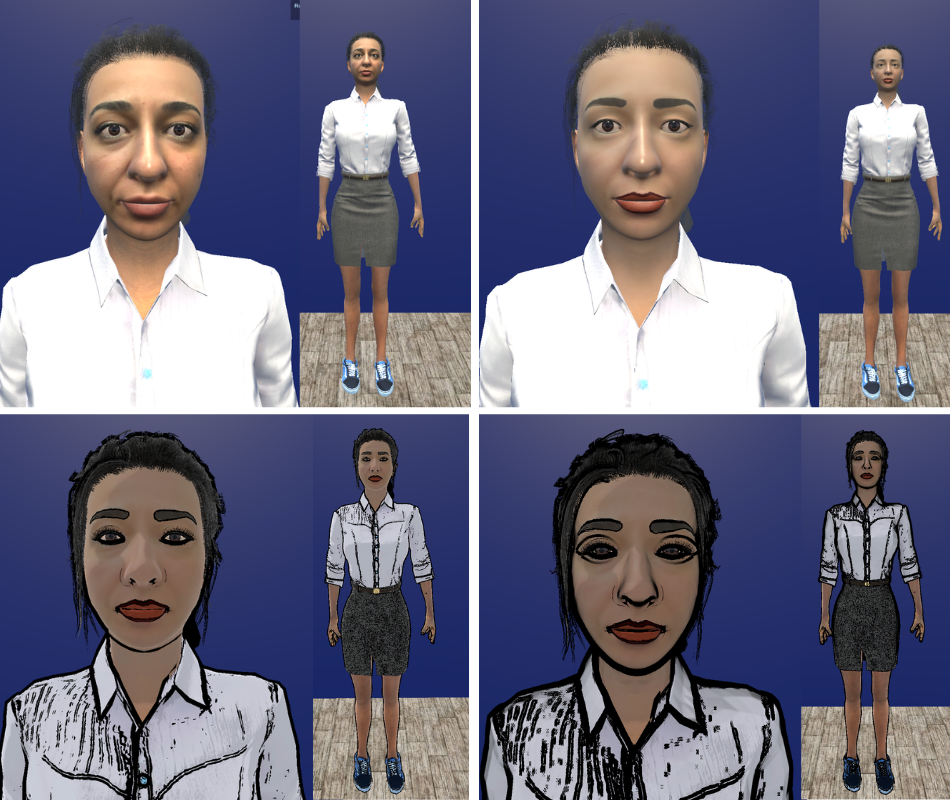
\includegraphics[width=0.86\textwidth, viewport=0 300 356.25 600, clip]{avaturn_best_1}\\[0.2em]
      \sn{Standard PBR, unmodified texture}
    \end{column}
    \begin{column}{0.32\textwidth}
      \centering
      \colorbox{knlight}{\parbox{0.9\textwidth}{\centering\small\color{knblue}\textbf{C3 — NPR}}}\\[0.4em]
      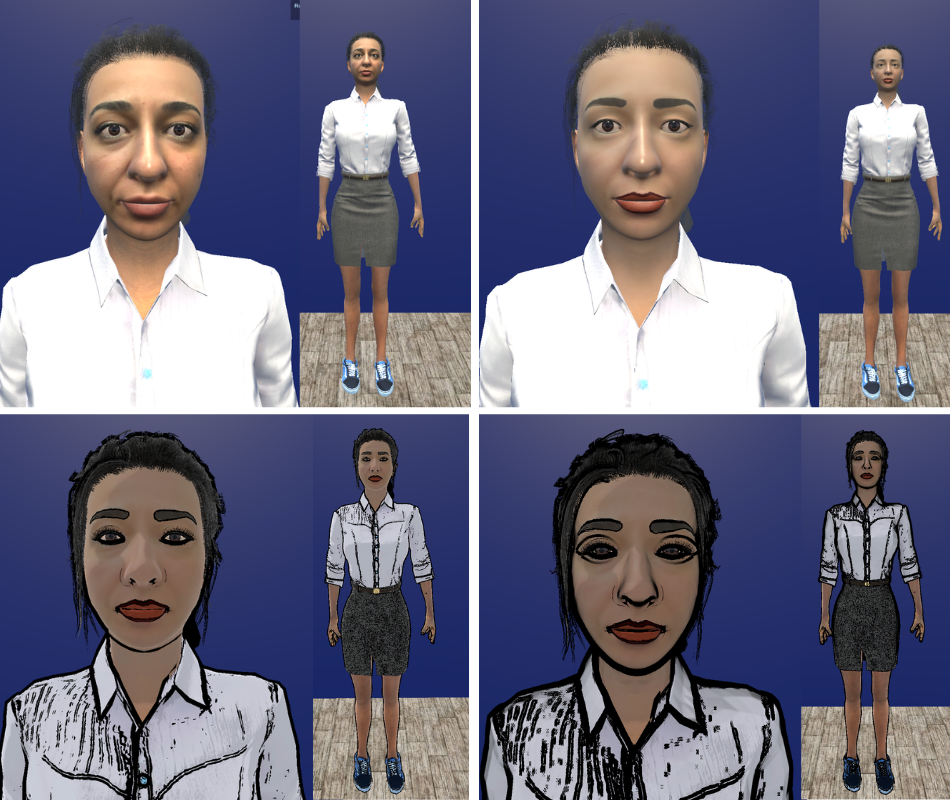
\includegraphics[width=0.86\textwidth, viewport=356.25 0 712.5 300, clip]{avaturn_best_1}\\[0.2em]
      \sn{Outline + X-Toon + Sobel,\\ preprocessed head texture}
    \end{column}
  \end{columns}
  \takeaway{C2 and C3 share identity, geometry, animation and voice. Only the rendering changes. That is the critical comparison.}
\end{frame}

%% ============================================================
%% PART 1 — PARAMETER ADJUSTMENT STUDY (RQ2)
%% ============================================================

\begin{frame}{Parameter adjustment study}{The composite was chosen by people, not by eye}
  \vspace{0.2em}
  \begin{columns}[T]
    \begin{column}{0.52\textwidth}
      \small
      \textbf{Design.} 45 participants ranked rendered variants by \hl{perceived trustworthiness}. Five rounds, one parameter group each. Borda count, Friedman omnibus, Wilcoxon on the top pair.
      \vspace{0.5em}

      \begin{tabular}{@{}llc@{}}
        \toprule
        \textbf{Round} & \textbf{Winner} & \textbf{Significant?} \\
        \midrule
        R1 inner threshold & 0.03 & no ($p=.31$) \\
        R2 outline width   & 0.003 & no ($p=.82$) \\
        R3 shadow / bias   & 0.5 / 1.0 & no ($p=.53$) \\
        R4 Kuwahara        & \bad{none} & \good{yes ($p=.003$)} \\
        R5 Hierarchical    & \bad{none} & \good{yes ($p<.001$)} \\
        \bottomrule
      \end{tabular}
      \vspace{0.6em}

      \sn{R1 and R3 were settled by a separate visual appeal question.}
    \end{column}
    \begin{column}{0.46\textwidth}
      \centering
      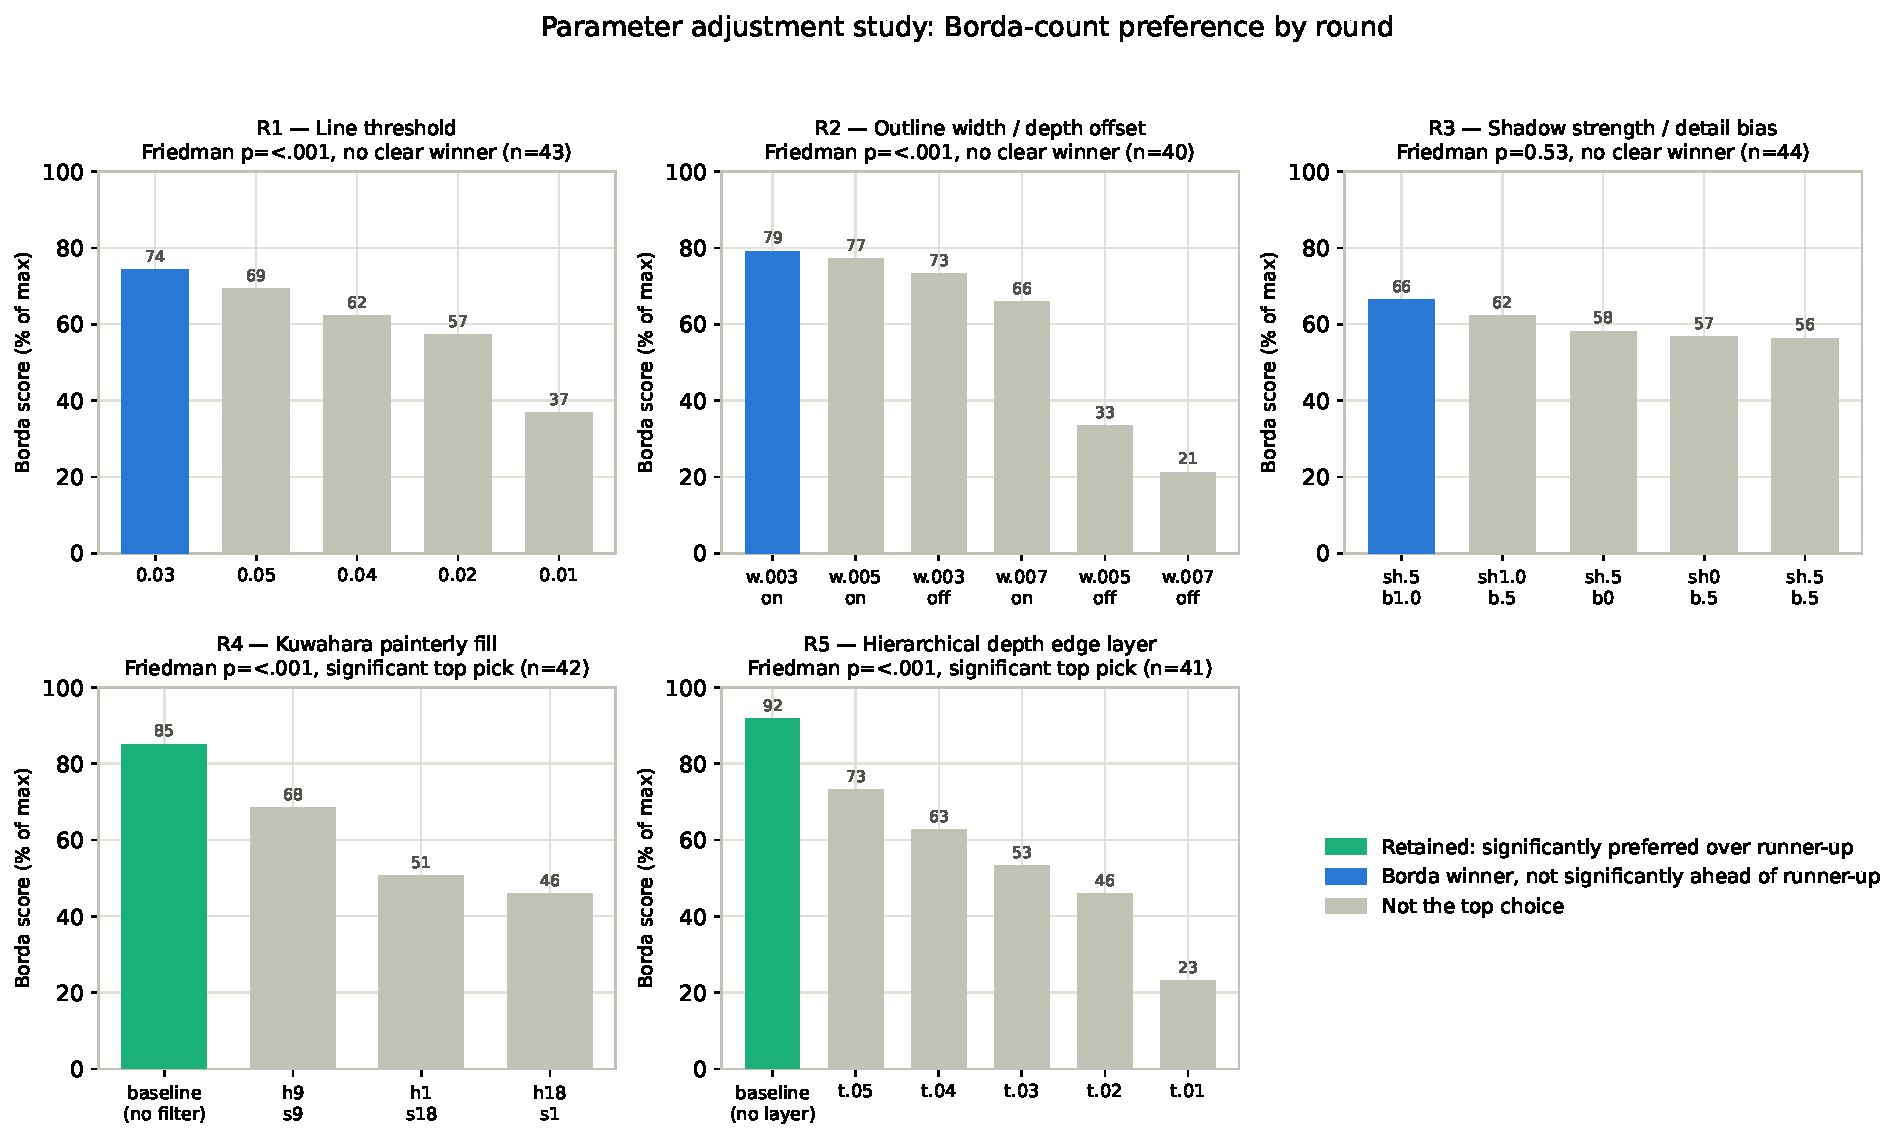
\includegraphics[width=\textwidth]{prestudy_summary}\\[0.1em]
      \sn{Borda score per round, \% of maximum}
    \end{column}
  \end{columns}
  \takeaway{Participants significantly \emph{preferred no post-processing}. Kuwahara and the hierarchical layer were both removed. RQ2's answer is a three-part composite plus head texture preprocessing.}
\end{frame}

%% ============================================================
%% PART 2 — MAIN USER STUDY: DESIGN
%% ============================================================

\begin{frame}{Main user study}{Within-subjects, video based}
  \vspace{0.2em}
  \begin{columns}[T]
    \begin{column}{0.50\textwidth}
      \small
      \textbf{Task.} Read a decision vignette, watch an advisor recommend one option, then rate the advisor. Three times, once per condition.
      \vspace{0.5em}

      \textbf{Scenarios.} Career choice, travel route, learning resource. Each targets a different trust dimension. Recommended option and discussion order alternate.
      \vspace{0.5em}

      \textbf{Counterbalancing.} $3\times3$ Latin square, three study versions.
      \vspace{0.5em}

      \textbf{Sample.} 52 enrolled, 11 excluded on gating checks, \hl{$n=41$} complete.\\
      Age $M=27.6$ ($SD=5.4$); 23 women, 17 men, 1 non-binary.
    \end{column}
    \begin{column}{0.48\textwidth}
      \small
      \textbf{Measures per video block}
      \vspace{0.3em}
      \begin{tabular}{@{}llc@{}}
        \toprule
        \textbf{Subscale} & \textbf{Source} & \textbf{$\alpha$} \\
        \midrule
        Likeability & Godspeed & .94 \\
        Eeriness    & Ho \& MacDorman & .87 \\
        Ability     & Mayer et al. & .96 \\
        Benevolence & Mayer et al. & .95 \\
        Integrity   & Mayer et al. & .92 \\
        \bottomrule
      \end{tabular}
      \vspace{0.6em}

      \textbf{After all three blocks}
      \begin{itemize}
        \item[] \small Forced ranking: who would you consult, who is most trustworthy, who is least unsettling.
      \end{itemize}
      \vspace{0.3em}
      \sn{All subscales exceeded $\alpha=.70$ overall and within every condition.}
    \end{column}
  \end{columns}
\end{frame}

\begin{frame}{Four hypotheses}
  \vspace{0.6em}
  \small
  \begin{tabular}{@{}p{0.055\textwidth}p{0.60\textwidth}p{0.29\textwidth}@{}}
    \toprule
    & \textbf{Prediction} & \textbf{Test} \\
    \midrule
    \textbf{H1} & NPR (C3) is rated \emph{less eerie} than the photorealistic avatar (C2). & RM-ANOVA, Holm pairwise \\
    \addlinespace
    \textbf{H2} & NPR (C3) does \emph{not} cost trust relative to C2. & Pairwise \textbf{plus} TOST equivalence, $d=0.3$ bound \\
    \addlinespace
    \textbf{H3} & Eeriness lowers trust and likeability raises it, within each participant. & Person-centred multilevel regression \\
    \addlinespace
    \textbf{H4} & NPR (C3) does \emph{not} cost trust relative to the real speaker (C1). & Same as H2, against C1 \\
    \bottomrule
  \end{tabular}
  \vspace{1.0em}

  \colorbox{knlight}{\parbox{0.97\textwidth}{\small\color{knblue}
  H2 and H4 predict a \textbf{null}. A non-significant $p$ is not evidence of equivalence, so both also carry a pre-specified TOST equivalence test.}}
\end{frame}

%% ============================================================
%% PART 3 — RESULTS
%% ============================================================

\begin{frame}{Manipulation check}{Did participants actually see a difference?}
  \vspace{0.2em}
  \begin{columns}[T]
    \begin{column}{0.44\textwidth}
      \vspace{0.4em}
      \centering
      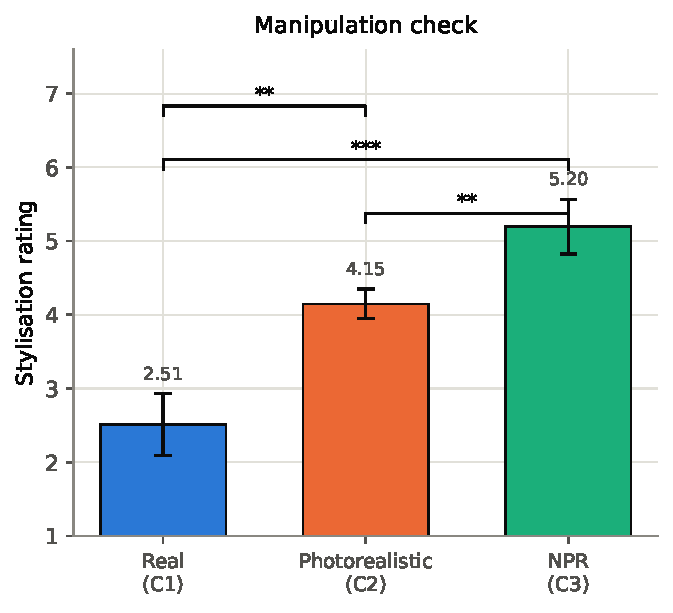
\includegraphics[height=0.62\textheight]{fig_manipulation_check}
    \end{column}
    \begin{column}{0.54\textwidth}
      \vspace{0.8em}
      \small
      Part H asked how stylised each advisor looked, from 1 (completely realistic) to 7 (very stylised).
      \vspace{0.6em}

      \begin{tabular}{@{}ll@{}}
        \toprule
        Omnibus & $F(2,80)=15.45$, $p<.001$, $\eta^2_p=.28$ \\
        \midrule
        C1 vs C2 & $p=.001$, $g=0.87$ \\
        C1 vs C3 & $p<.001$, $g=1.23$ \\
        C2 vs C3 & \good{$p=.004$, $g=0.55$} \\
        \bottomrule
      \end{tabular}
      \vspace{0.8em}

      Ratings rise monotonically from Real to Photorealistic to NPR. All three conditions separate.
    \end{column}
  \end{columns}
  \vspace{-0.4em}
  \takeaway{The manipulation worked. No null result below can be blamed on participants not noticing the rendering.}
\end{frame}

\begin{frame}{All five subscales at once}
  \vspace{0.3em}
  \begin{center}
    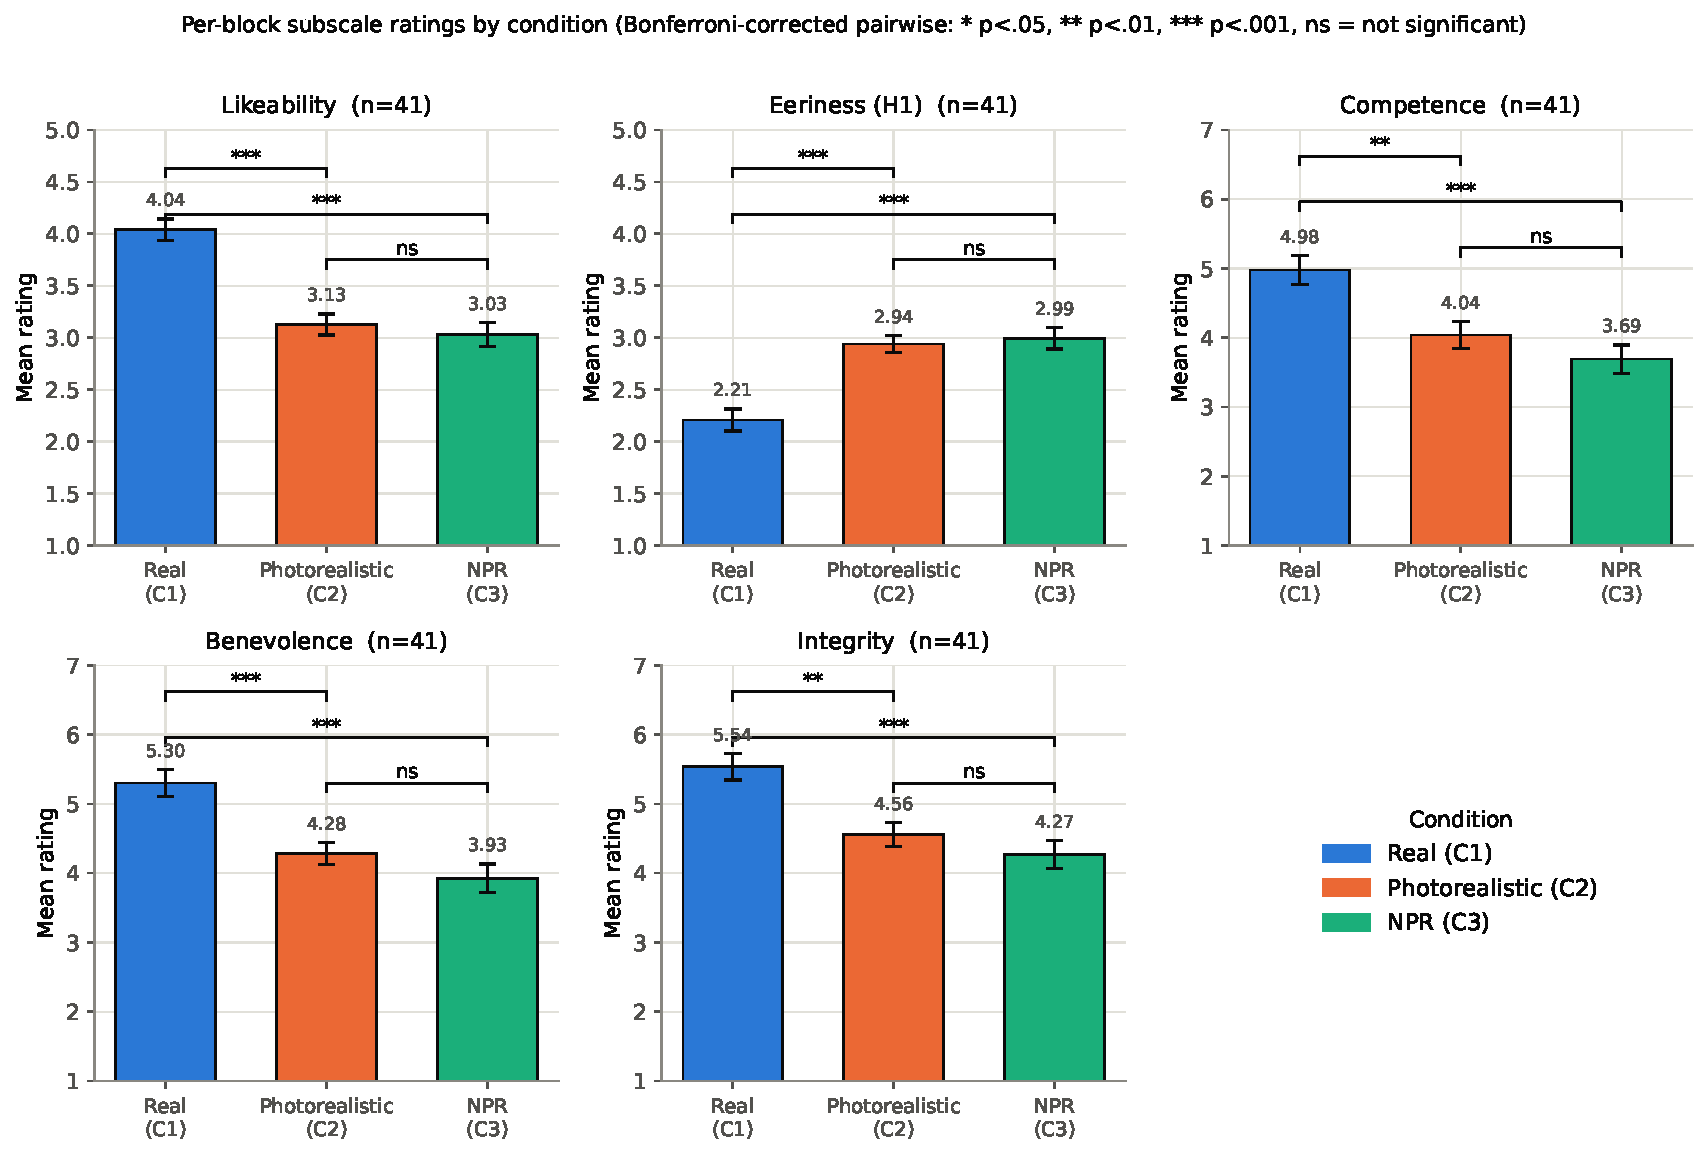
\includegraphics[height=0.635\textheight]{fig_subscales_grid}
  \end{center}
  \vspace{-0.3em}
  \begin{columns}[T]
    \begin{column}{0.49\textwidth}
      \footnotesize \textbf{\color{knblue}The real speaker separates from both avatars on every subscale.}
    \end{column}
    \begin{column}{0.49\textwidth}
      \footnotesize \textbf{\color{knblue}The two avatars separate from each other on \emph{none} of them.}
    \end{column}
  \end{columns}
\end{frame}

\begin{frame}{H1 — Does NPR reduce eeriness?}
  \vspace{0.3em}
  \begin{columns}[T]
    \begin{column}{0.55\textwidth}
      \small
      \begin{tabular}{@{}lccc@{}}
        \toprule
        \textbf{Eeriness} & \textbf{C1 vs C2} & \textbf{C1 vs C3} & \textbf{C2 vs C3} \\
        \midrule
        $p$ & $<.001$ & $<.001$ & \bad{$.66$} \\
        $g$ & $0.98$ & $0.98$ & \bad{$0.07$} \\
        \bottomrule
      \end{tabular}
      \vspace{0.4em}

      \sn{Omnibus: $F(2,80)=20.39$, $p<.001$, $\eta^2_p=.34$}
      \vspace{1.0em}

      \begin{itemize}
        \item Eeriness rose from C1 to C2 to C3, the \hl{opposite} of the prediction.
        \item The real speaker differed from both avatars.
        \item The two avatars were \hl{statistically indistinguishable}. Effect size $g=0.07$ is essentially zero.
      \end{itemize}
    \end{column}
    \begin{column}{0.43\textwidth}
      \vspace{1.2em}
      \begin{center}
        \verdict{knred}{\ H1 NOT SUPPORTED\ }
      \end{center}
      \vspace{0.8em}
      \colorbox{knlight}{\parbox{0.95\textwidth}{\small\color{knblue}
      Participants \emph{saw} the stylisation, as the manipulation check confirmed. They just did not find it \emph{less eerie}.\\[0.5em]
      Stylisation and eeriness turn out to be separate effects here.}}
    \end{column}
  \end{columns}
\end{frame}

\begin{frame}{H2 — Does NPR cost trust against the photorealistic avatar?}
  \vspace{0.2em}
  \begin{columns}[T]
    \begin{column}{0.52\textwidth}
      \small
      \textbf{Step 1. Pairwise comparisons, C2 vs C3}
      \vspace{0.3em}

      \begin{tabular}{@{}lcc@{}}
        \toprule
        & $p$ & $g$ \\
        \midrule
        Ability      & $.21$ & $0.20$ \\
        Benevolence  & $.18$ & $0.19$ \\
        Integrity    & $.27$ & $0.16$ \\
        \bottomrule
      \end{tabular}
      \vspace{0.7em}

      \textbf{Step 2. TOST equivalence, trust composite}
      \vspace{0.3em}

      \begin{tabular}{@{}lccc@{}}
        \toprule
        & Diff. & Bound & TOST $p$ \\
        \midrule
        C2 vs C3 & $0.33$ & $\pm0.51$ & \bad{$.240$} \\
        \bottomrule
      \end{tabular}
      \vspace{0.6em}

      \sn{Realised power near $0.20$ at $n=41$.}
    \end{column}
    \begin{column}{0.46\textwidth}
      \centering
      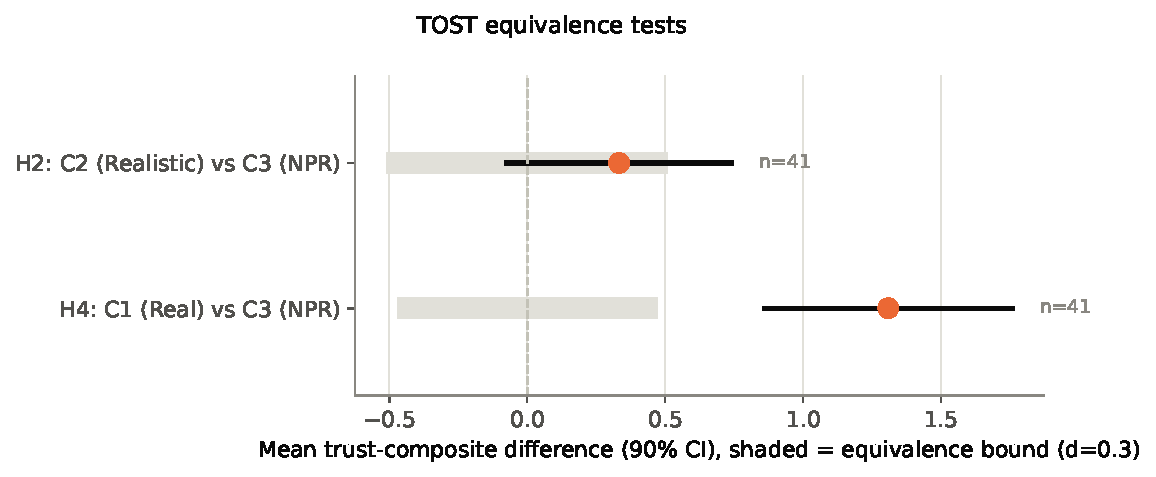
\includegraphics[width=0.95\textwidth]{fig_tost_equivalence}
    \end{column}
  \end{columns}
  \vspace{-0.4em}
  \begin{center}
    \verdict{knaccent}{\ H2 INCONCLUSIVE\ }\enspace
    {\footnotesize No difference detected, but equivalence not established either.\\ Roughly \hl{three times} the sample is needed to separate the two.}
  \end{center}
\end{frame}

\begin{frame}{H3 — Eeriness, likeability and trust}
  \vspace{0.2em}
  \begin{columns}[T]
    \begin{column}{0.60\textwidth}
      \centering
      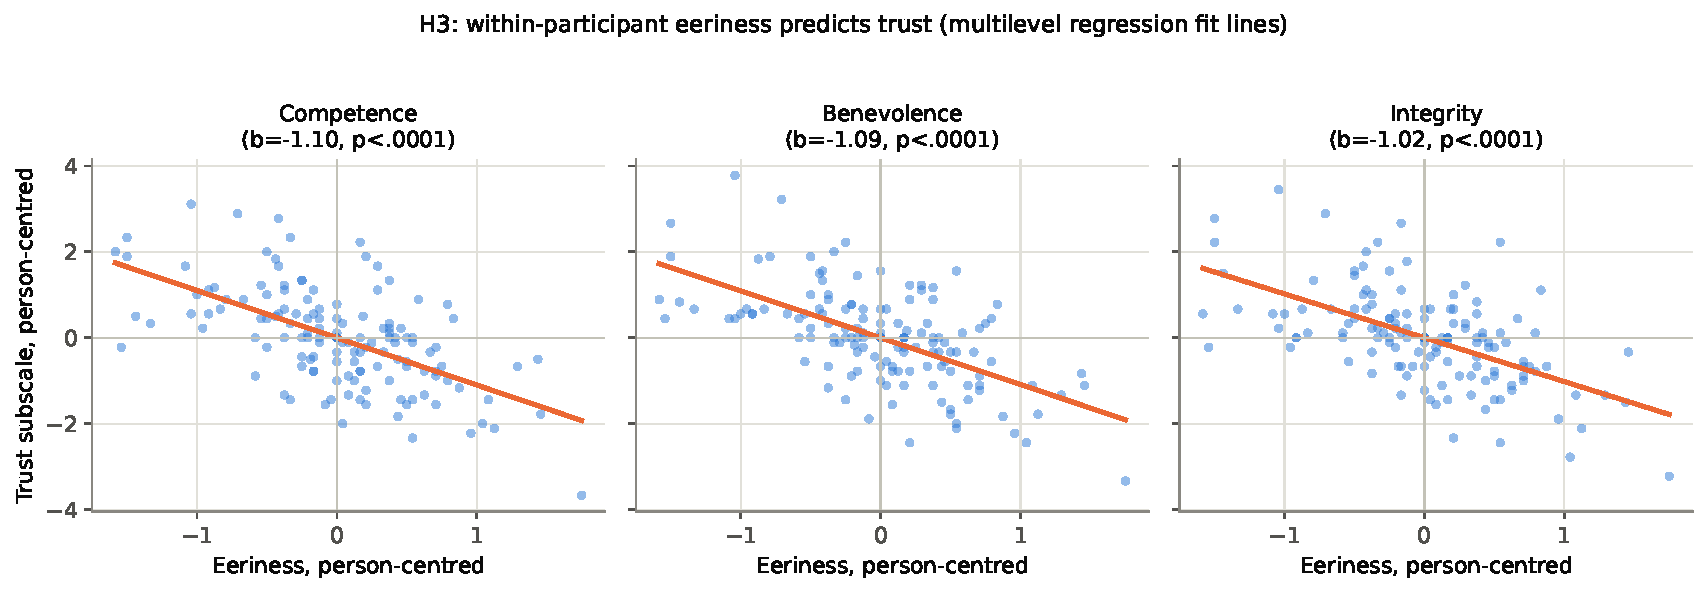
\includegraphics[height=0.60\textheight]{fig_h3_eeriness_trust}
    \end{column}
    \begin{column}{0.38\textwidth}
      \vspace{0.3em}
      \footnotesize
      \begin{tabular}{@{}lcc@{}}
        \toprule
        & \textbf{Eeriness} & \textbf{Likeability} \\
        \midrule
        Ability      & $-1.17$ & $+1.10$ \\
        Benevolence  & $-1.10$ & $+1.10$ \\
        Integrity    & $-1.02$ & $+1.08$ \\
        \bottomrule
      \end{tabular}\\[0.2em]
      {\color{kngrey}\scriptsize Fixed-effect slopes, all $p<.001$}
      \vspace{0.6em}

      \begin{center}\verdict{kngreen}{\ H3 CONFIRMED\ }\end{center}
      \vspace{0.4em}

      One point more eeriness costs about one point of trust, on every dimension. Likeability lifts it by the same amount.
      \vspace{0.3em}

      {\color{kngrey}\scriptsize Caveat: the two correlate at $r=-.72$ within participants and cannot be separated cleanly here.}
    \end{column}
  \end{columns}
  \vspace{-0.6em}
  \takeaway{The route from appearance to trust is open. The composite never travelled it.}
\end{frame}

\begin{frame}{H4 — Does NPR reach the real human speaker?}
  \vspace{0.4em}
  \begin{columns}[T]
    \begin{column}{0.53\textwidth}
      \small
      \textbf{Pairwise, C1 vs C3.} Ability, benevolence and integrity were \hl{all significantly higher} for the real speaker ($p<.001$, $g=0.75$ to $0.80$).
      \vspace{0.8em}

      \textbf{TOST equivalence, trust composite}
      \vspace{0.3em}

      \begin{tabular}{@{}lccc@{}}
        \toprule
        & Diff. & Bound & TOST $p$ \\
        \midrule
        C1 vs C3 & \bad{$1.31$} & $\pm0.47$ & $.998$ \\
        \bottomrule
      \end{tabular}
      \vspace{0.8em}

      The difference is nearly \hl{three times} the equivalence bound. This is not a marginal shortfall.
    \end{column}
    \begin{column}{0.45\textwidth}
      \vspace{1.0em}
      \begin{center}
        \verdict{knred}{\ H4 NOT SUPPORTED\ }
      \end{center}
      \vspace{0.9em}
      \colorbox{knlight}{\parbox{0.95\textwidth}{\small\color{knblue}
      Two explanations stay open and this design cannot separate them:\\[0.5em]
      1.\ The uncanny valley predicts exactly this gap.\\[0.3em]
      2.\ Some participants may have recognised the speaker, who is the researcher.}}
    \end{column}
  \end{columns}
\end{frame}

\begin{frame}{The behavioural measure}{Forced ranking after all three videos}
  \vspace{0.2em}
  \begin{center}
    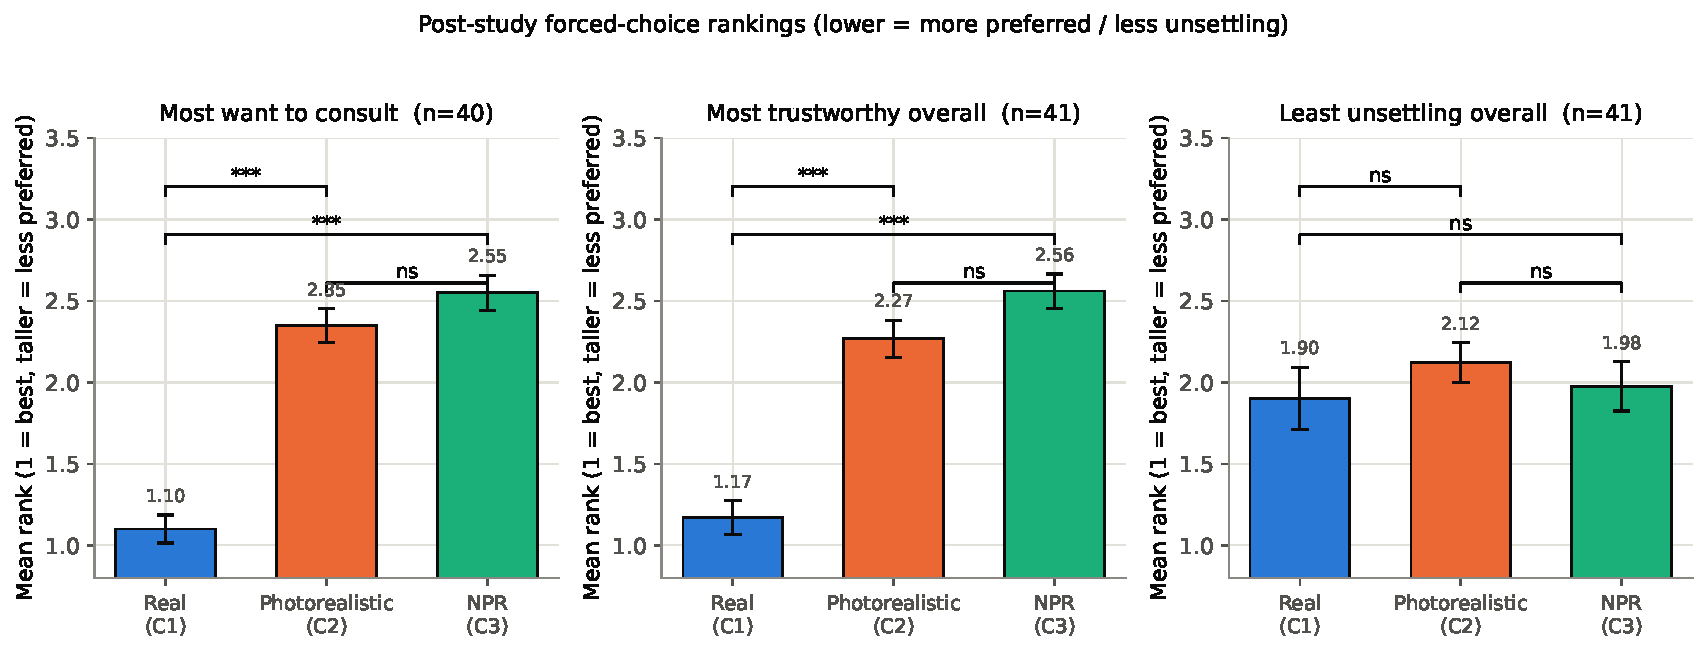
\includegraphics[height=0.485\textheight]{fig_rankings}
  \end{center}
  \vspace{-0.2em}
  \begin{columns}[T]
    \begin{column}{0.62\textwidth}
      \scriptsize
      \begin{tabular}{@{}llll@{}}
        \toprule
        \textbf{Question} & \textbf{Friedman} & \textbf{C1 vs C2/C3} & \textbf{C2 vs C3} \\
        \midrule
        Most want to consult & $\chi^2_F(2)=49.40$, $p<.001$ & $p<.001$ & $p=.21$ \\
        Most trustworthy     & $\chi^2_F(2)=44.05$, $p<.001$ & $p<.001$ & $p=.07$ \\
        Least unsettling     & $\chi^2_F(2)=1.02$, $p=.60$   & $p=.97$  & $p=.97$ \\
        \bottomrule
      \end{tabular}
    \end{column}
    \begin{column}{0.36\textwidth}
      \scriptsize
      Canales et al.\ found ratings and behaviour \emph{diverge}. Here they \hl{converged}. C3 attracted no more behavioural endorsement than C2.
    \end{column}
  \end{columns}
\end{frame}

\begin{frame}{Robustness checks}{Three ways the null could have been an artefact, and was not}
  \vspace{0.6em}
  \begin{columns}[T]
    \begin{column}{0.315\textwidth}
      \colorbox{knlight}{\parbox{0.93\textwidth}{\small\color{knblue}\textbf{Order effects}}}\\[0.5em]
      \small Video position had no significant effect on any subscale. Likeability came closest at $p=.054$.
      \vspace{0.4em}

      \sn{Study version groups differed on likeability and eeriness, but on no trust subscale. That comparison is between subjects.}
    \end{column}
    \begin{column}{0.315\textwidth}
      \colorbox{knlight}{\parbox{0.93\textwidth}{\small\color{knblue}\textbf{Suspicion}}}\\[0.5em]
      \small 24 of 41 named realism, stylisation or trust when asked what the study was about.
      \vspace{0.4em}

      Re-running H1 and H2 on the remaining 17 did not change the pattern.
      \vspace{0.4em}

      \sn{Participants answered on their own impressions, not on a guessed hypothesis.}
    \end{column}
    \begin{column}{0.315\textwidth}
      \colorbox{knlight}{\parbox{0.93\textwidth}{\small\color{knblue}\textbf{Secondary measures}}}\\[0.5em]
      \small Agreement with the recommendation did not differ by condition, $F(2,80)=2.10$, $p=.13$.
      \vspace{0.4em}

      Dispositional trust did not predict the trust composite, $r(39)=-.10$, $p=.52$.
      \vspace{0.4em}

      \sn{Preference shift was rare everywhere: 4, 5 and 1 of 41.}
    \end{column}
  \end{columns}
\end{frame}

%% ============================================================
%% PART 4 — DISCUSSION
%% ============================================================

\begin{frame}{Discussion}{Two patterns that need explaining}
  \vspace{1.0em}
  \begin{columns}[T]
    \begin{column}{0.48\textwidth}
      \colorbox{knlight}{\parbox{0.95\textwidth}{\small\color{knblue}\textbf{Pattern 1}\\[0.4em]
      The real speaker sits far above both avatars, on every subscale and both significant rankings.}}
    \end{column}
    \begin{column}{0.48\textwidth}
      \colorbox{knlight}{\parbox{0.95\textwidth}{\small\color{knblue}\textbf{Pattern 2}\\[0.4em]
      The two avatars looked different to participants, yet scored identically on everything that mattered.}}
    \end{column}
  \end{columns}
  \vspace{1.4em}
  \begin{center}
    \small And one constraint on any explanation:\\[0.5em]
    {\color{knblue}\textbf{Eeriness and likeability \emph{did} predict trust (H3). The road was open.}}\\[0.4em]
    {\color{knblue}\textbf{The composite changed what people saw without travelling it.}}
  \end{center}
\end{frame}

\begin{frame}{Why eeriness did not fall}{Two mismatches inside the composite}
  \vspace{0.4em}
  \begin{columns}[T]
    \begin{column}{0.48\textwidth}
      \textbf{\color{knblue}1. Material versus shape}
      \vspace{0.4em}
      \small
      \begin{itemize}
        \item The composite stylises the \hl{material} and leaves the \hl{shape} untouched.
        \item Zell et al.: material drives eeriness, so this should have helped.
        \item But the same work reports eeriness \hl{rises} when material and shape disagree in stylisation level.
        \item C3 is exactly that case: a stylised surface on a photogrammetric face.
      \end{itemize}
      \vspace{0.3em}
      \sn{The abstraction may have removed one source of eeriness while adding another.}
    \end{column}
    \begin{column}{0.48\textwidth}
      \textbf{\color{knblue}2. Appearance versus performance}
      \vspace{0.4em}
      \small
      \begin{itemize}
        \item Both avatars inherit the \hl{same} recorded human voice, gaze and lip animation.
        \item C3 therefore pairs a fully human performance with a visibly abstracted face.
        \item Cihodaru-Ştefanache \& Podina: uncanniness arises from features perceived at \hl{inconsistent} levels of anthropomorphism.
        \item A shading operator changes appearance only. It could only widen that gap.
      \end{itemize}
    \end{column}
  \end{columns}
\end{frame}

\begin{frame}{Three more explanations on the table}
  \vspace{0.5em}
  \small
  \begin{columns}[T]
    \begin{column}{0.315\textwidth}
      \textbf{\color{knblue}The comparison set}
      \vspace{0.4em}
      \begin{itemize}
        \item[] Once a real person anchors the top of the scale, the only judgement left is \emph{how far below}.
        \item[] Both avatars were recognisably CG. A rendering difference competes against a categorical one.
        \item[] C3 followed C1 directly in two versions of three. C2 never did.
      \end{itemize}
    \end{column}
    \begin{column}{0.315\textwidth}
      \textbf{\color{knblue}Generative AI expectations}
      \vspace{0.4em}
      \begin{itemize}
        \item[] One participant asked afterwards \emph{which AI system generated the videos}.
        \item[] Nothing in the materials ruled that reading out.
        \item[] Scepticism towards machine-made media depresses \emph{both} avatars equally.
      \end{itemize}
    \end{column}
    \begin{column}{0.315\textwidth}
      \textbf{\color{knblue}The video setting}
      \vspace{0.4em}
      \begin{itemize}
        \item[] Flat screen, prerecorded, no interaction, no shared space.
        \item[] Zibrek et al.\ found render style significantly moved presence in VR.
        \item[] What is too weak in a browser window may register once the avatar shares your room.
      \end{itemize}
    \end{column}
  \end{columns}
\end{frame}

%% ============================================================
%% PART 5 — LIMITATIONS
%% ============================================================

\begin{frame}{Limitations}
  \vspace{0.5em}
  \small
  \begin{columns}[T]
    \begin{column}{0.48\textwidth}
      \colorbox{knlight}{\parbox{0.95\textwidth}{\color{knblue}\textbf{Session length}}}\\[0.5em]
      Both studies had to fit 10 to 15 minutes, and every measure was repeated three times. That capped how many measures and conditions were affordable.
      \vspace{0.9em}

      \colorbox{knlight}{\parbox{0.95\textwidth}{\color{knblue}\textbf{One configuration only}}}\\[0.5em]
      One composite, one avatar identity, one platform, three scenarios. The findings describe \hl{this configuration}, not NPR as a category.
    \end{column}
    \begin{column}{0.48\textwidth}
      \colorbox{knlight}{\parbox{0.95\textwidth}{\color{knblue}\textbf{Sample size}}}\\[0.5em]
      The submission deadline set the collection window, which fell in the semester break. $n=41$ met the power requirement for \emph{detecting} a difference, not the far larger one \emph{equivalence} demands.
      \vspace{0.9em}

      \colorbox{knlight}{\parbox{0.95\textwidth}{\color{knblue}\textbf{Counterbalancing}}}\\[0.5em]
      Three conditions need six orders for a full design. That needs roughly twice the sample, so three orders were used.
      \vspace{0.4em}

      \sn{The parameter study also tested only the highest-impact groups, so the composite is suitable rather than globally optimal.}
    \end{column}
  \end{columns}
\end{frame}

%% ============================================================
%% PART 6 — CONCLUSION
%% ============================================================

\begin{frame}{Conclusion}{What the three questions ended up answering}
  \vspace{0.4em}
  \small
  \begin{block}{\textbf{RQ1} \enspace Adaptation across platforms}
    All eight techniques ran on all three platforms. The dividing line is whether an operator needs \hl{new parameter values}, which is always possible, or a \hl{new input signal}, which only an open pipeline provides.
  \end{block}
  \begin{block}{\textbf{RQ2} \enspace Best balance of abstraction and legibility}
    No technique reached it by rendering alone on a photogrammetric avatar. The answer is a \hl{three-part composite}, outline plus X-Toon plus Sobel, \hl{paired with head texture preprocessing}.
  \end{block}
  \begin{block}{\textbf{RQ3} \enspace Effect on eeriness and trust}
    H1 not supported, H2 inconclusive, \good{H3 confirmed}, H4 not supported. The composite did not lower eeriness, and it also carried \hl{no observed trust penalty}.
  \end{block}
  \vspace{0.2em}
  \begin{center}
    \colorbox{knlight}{\parbox{0.95\textwidth}{\centering\color{knblue}\footnotesize\textbf{A developer choosing the stylised version need not assume a disadvantage.\\ The real distance is not between two render styles. It is to the actual human.}}}
  \end{center}
\end{frame}

\begin{frame}{Future work}
  \vspace{0.6em}
  \small
  \begin{columns}[T]
    \begin{column}{0.48\textwidth}
      \textbf{\color{knblue}Settle the open question}
      \begin{itemize}
        \item Repeat C2 versus C3 with roughly \hl{120 participants}. Inside the bound confirms no trust cost, outside exposes one too small to see here.
      \end{itemize}
      \vspace{0.8em}

      \textbf{\color{knblue}Test the competing explanations}
      \begin{itemize}
        \item Extend abstraction to the \hl{geometry}, not just the material.
        \item Drop the real speaker and let the two avatars be compared alone.
        \item State up front that the videos are \hl{not AI-generated}.
      \end{itemize}
    \end{column}
    \begin{column}{0.48\textwidth}
      \textbf{\color{knblue}Replace the point with a curve}
      \begin{itemize}
        \item Sweep abstraction strength continuously instead of testing one setting. That traces how eeriness and trust move together and can reveal an optimum between the extremes.
      \end{itemize}
      \vspace{0.8em}

      \textbf{\color{knblue}Restore what video removed}
      \begin{itemize}
        \item Interaction and shared space, in VR.
      \end{itemize}
      \vspace{0.6em}

      \textbf{\color{knblue}Widen the sample of avatars}
      \begin{itemize}
        \item Multiple identities and platforms, to separate a general effect from one specific to this face.
      \end{itemize}
    \end{column}
  \end{columns}
\end{frame}

\begin{frame}[plain]
  \vspace{2.2em}
  \begin{center}
    {\LARGE\bfseries\color{knblue} Thank you}\\[1.2em]
    {\large\color{kngrey} Questions}\\[2.0em]
    \colorbox{knlight}{\parbox{0.78\textwidth}{\centering\color{knblue}\small
    Eight NPR techniques, three avatar platforms, two studies, 86 participants.\\[0.6em]
    Stylisation was clearly seen, cost no measurable trust,\\ and did not close the gap to a real human.}}\\[1.6em]
    {\footnotesize\color{kngrey} Nidanur Günay \quad|\quad nidanur.guenay@uni-konstanz.de}
  \end{center}
\end{frame}

%% ============================================================
%% BACKUP SLIDES
%% ============================================================

\begin{frame}[plain]
  \vspace{3.0em}
  \begin{center}
    {\Large\color{kngrey} Backup slides}
  \end{center}
\end{frame}

\begin{frame}{Backup — Visual quality assessment of all eight techniques}
  \vspace{0.3em}
  \scriptsize
  \begin{tabular}{@{}lllllc@{}}
    \toprule
    \textbf{Technique} & \textbf{Facial} & \textbf{Temporal} & \textbf{Artefacts} & \textbf{Abstraction} & \textbf{Candidate} \\
    \midrule
    V1 Outline        & yes & yes & after tuning & \bad{not alone} & yes \\
    V2 Toon           & yes & yes & yes & \bad{no interior lines} & --- \\
    V2.2 X-Toon       & yes & yes & yes & manual mode chosen & yes \\
    V3 Normal edge    & \bad{landmarks missed} & yes & yes & yes & --- \\
    V4 Sobel          & after tuning & after tuning & after preprocessing & yes & yes \\
    V4.2 Gauss Sobel  & \bad{no gain over V4} & after tuning & yes & yes & --- \\
    V5 Hierarchical   & \bad{segments unclear} & yes & \bad{nose bridge artefact} & yes & yes \\
    V6 Kuwahara       & \bad{fails at large radius} & yes & yes & yes & yes \\
    \bottomrule
  \end{tabular}
  \vspace{0.8em}

  \sn{Five of the eight became candidates for the composite. The parameter adjustment study then removed V5 and V6, leaving V1, V2.2 and V4.}
\end{frame}

\begin{frame}{Backup — All variants shown in the parameter adjustment study}
  \vspace{0.2em}
  \begin{center}
    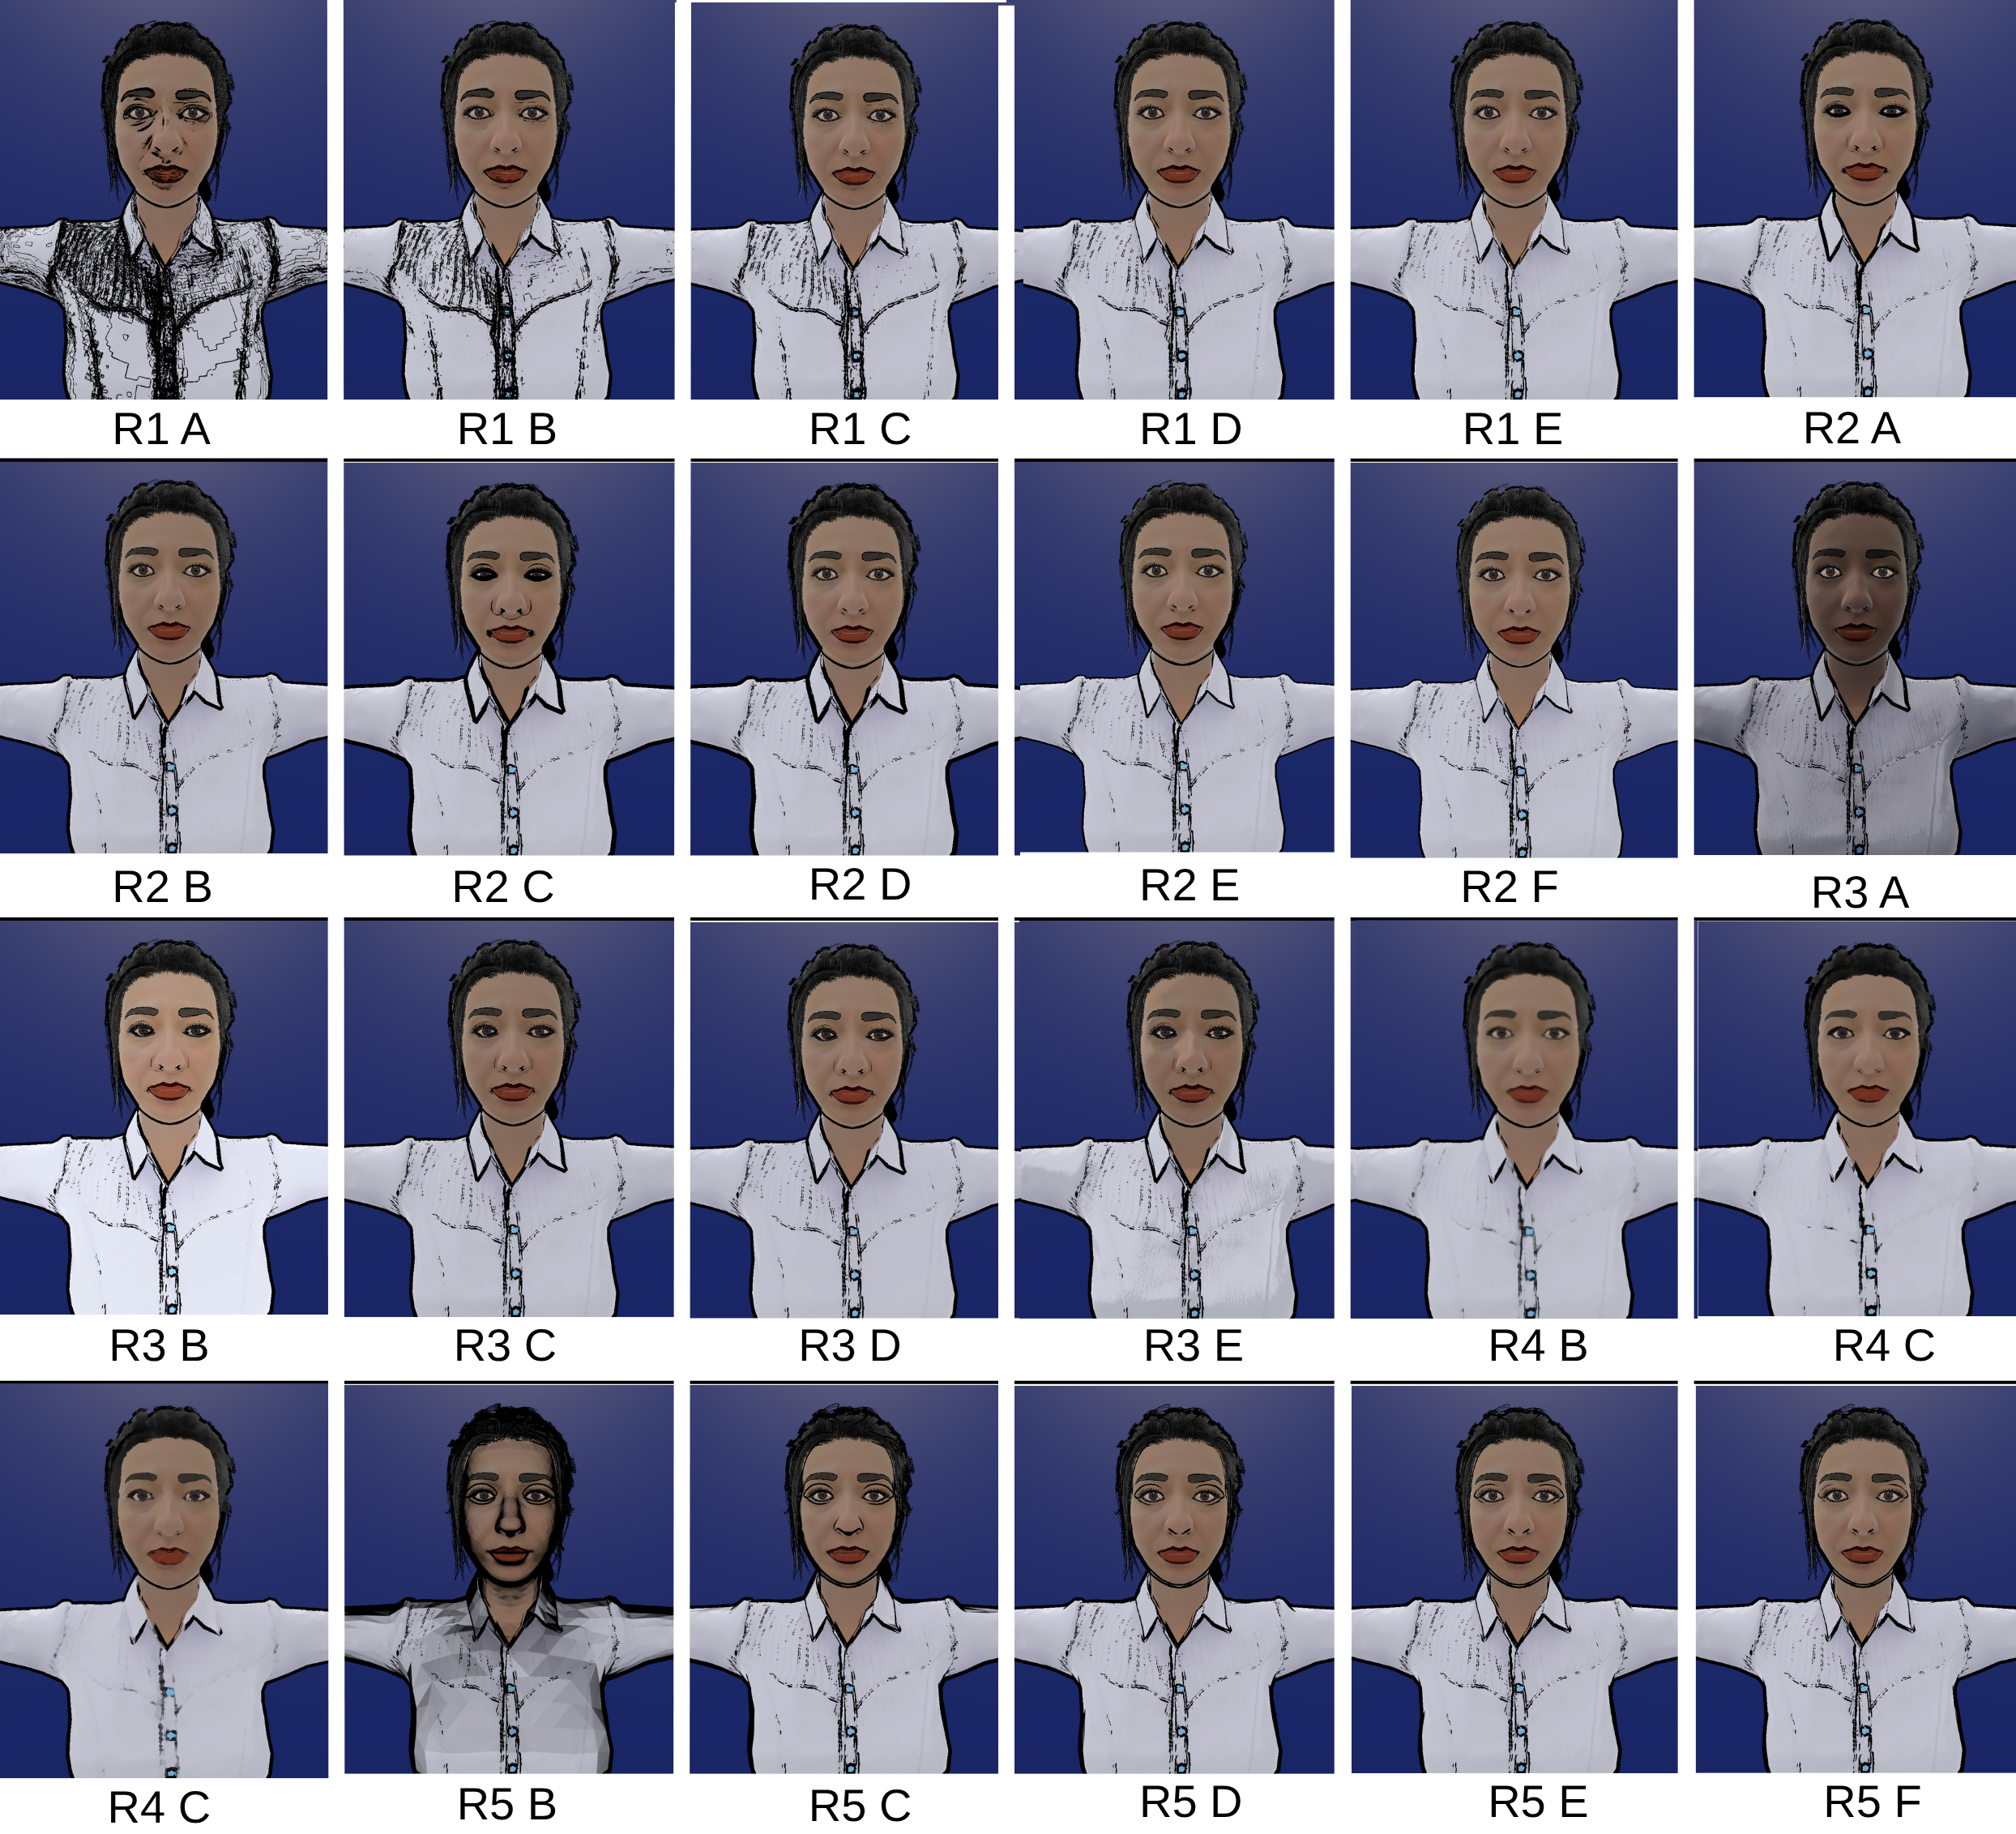
\includegraphics[height=0.78\textheight]{prestudy_all_versions}
  \end{center}
\end{frame}

\begin{frame}{Backup — Final composite parameters}
  \vspace{0.8em}
  \begin{columns}[T]
    \begin{column}{0.52\textwidth}
      \small
      \begin{tabular}{@{}lll@{}}
        \toprule
        \textbf{Parameter} & \textbf{Value} & \textbf{Source} \\
        \midrule
        Outline width            & 0.003 & R2 Borda winner \\
        Depth offset             & On    & R2 Borda winner \\
        Inner line threshold     & 0.05  & R1 appeal tiebreaker \\
        Shadow strength          & 0.0   & R3 appeal tiebreaker \\
        Detail bias              & 0.5   & R3 appeal tiebreaker \\
        Kuwahara filter          & \bad{Off} & R4 excluded ($p=.003$) \\
        Hierarchical layer       & \bad{Off} & R5 excluded ($p<.001$) \\
        \bottomrule
      \end{tabular}
    \end{column}
    \begin{column}{0.44\textwidth}
      \small
      \colorbox{knlight}{\parbox{0.95\textwidth}{\color{knblue}
      Three of the seven values came from a separate visual appeal question, since no configuration in those rounds was statistically ahead of its runner-up.}}
    \end{column}
  \end{columns}
\end{frame}

\begin{frame}{Backup — Eeriness against likeability}
  \vspace{0.3em}
  \begin{center}
    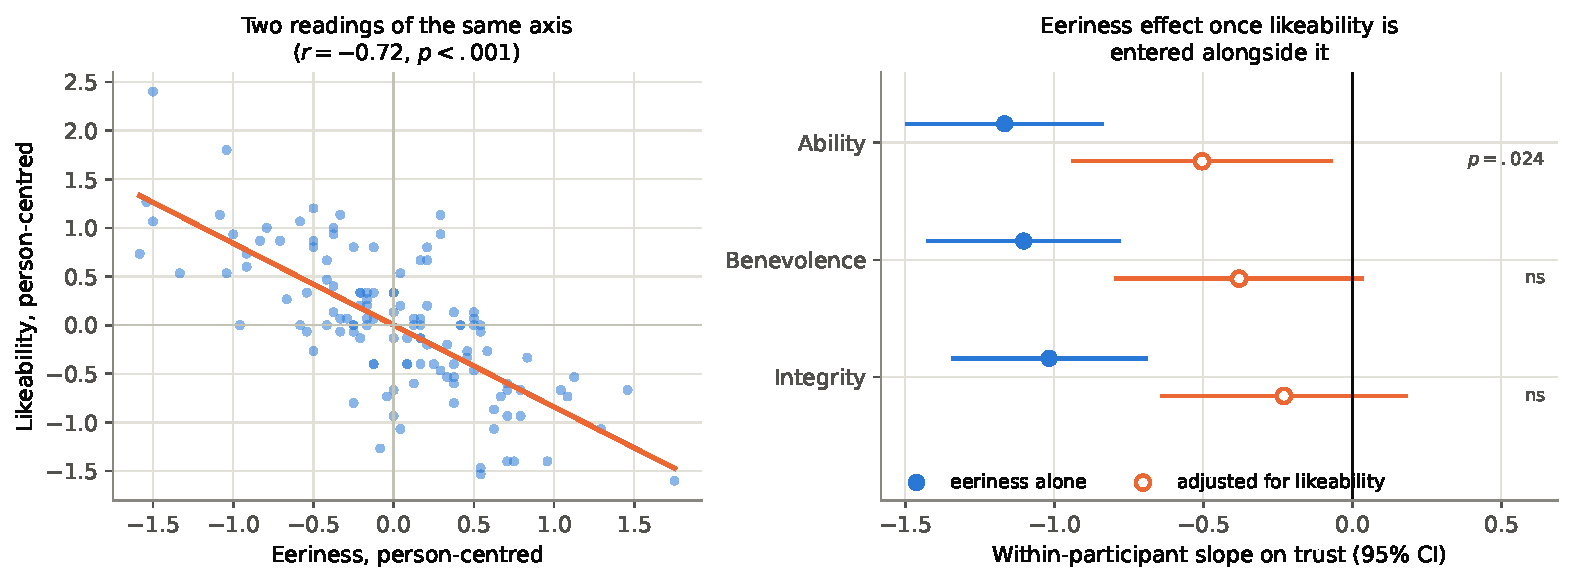
\includegraphics[width=0.95\textwidth]{fig_h3_likeability}
  \end{center}
  \vspace{-0.2em}
  \small Within participants the two correlate at $r=-.72$, sharing 52\% of their variance. Entering both in one model absorbs most of the eeriness effect: it survives on ability ($b=-0.50$, $p=.024$) but not benevolence ($p=.075$) or integrity ($p=.273$), while likeability holds on all three.
\end{frame}

\begin{frame}{Backup — Full statistics table}
  \vspace{0.5em}
  \scriptsize
  \begin{tabular}{lllll}
    \toprule
    \textbf{Subscale} & \textbf{Omnibus} & \textbf{C1 vs C2} & \textbf{C1 vs C3} & \textbf{C2 vs C3} \\
    \midrule
    Likeability  & $F(2,80)=26.85$, $p<.001$, $\eta^2_p=.40$ & $p<.001$, $g=0.92$ & $p<.001$, $g=1.02$ & $p=.54$, $g=0.08$ \\
    Eeriness     & $F(2,80)=20.39$, $p<.001$, $\eta^2_p=.34$ & $p<.001$, $g=0.98$ & $p<.001$, $g=0.98$ & $p=.66$, $g=0.07$ \\
    Ability      & $F(2,80)=10.91$, $p<.001$, $\eta^2_p=.21$ & $p=.004$, $g=0.53$ & $p<.001$, $g=0.75$ & $p=.21$, $g=0.20$ \\
    Benevolence  & $F(2,80)=14.31$, $p<.001$, $\eta^2_p=.26$ & $p<.001$, $g=0.59$ & $p<.001$, $g=0.79$ & $p=.18$, $g=0.19$ \\
    Integrity    & $F(2,80)=12.47$, $p<.001$, $\eta^2_p=.24$ & $p=.001$, $g=0.66$ & $p<.001$, $g=0.80$ & $p=.27$, $g=0.16$ \\
    \bottomrule
  \end{tabular}
  \vspace{1.2em}

  \normalsize
  \begin{columns}[T]
    \begin{column}{0.48\textwidth}
      \scriptsize
      \textbf{Order and version checks}\\[0.3em]
      \begin{tabular}{lcccc}
        \toprule
        & \multicolumn{2}{c}{Position} & \multicolumn{2}{c}{Study version} \\
        \textbf{Subscale} & $F(2,80)$ & $p$ & $F(2,38)$ & $p$ \\
        \midrule
        Likeability & $3.04$ & $.054$ & $\mathbf{7.07}$ & $\mathbf{.002}$ \\
        Eeriness    & $2.47$ & $.091$ & $\mathbf{5.57}$ & $\mathbf{.008}$ \\
        Ability     & $1.32$ & $.274$ & $1.23$ & $.304$ \\
        Benevolence & $2.10$ & $.130$ & $1.26$ & $.296$ \\
        Integrity   & $1.72$ & $.186$ & $2.04$ & $.144$ \\
        \bottomrule
      \end{tabular}
    \end{column}
    \begin{column}{0.48\textwidth}
      \scriptsize
      \textbf{Intraclass correlations, H3 models}\\[0.3em]
      Eeriness models: $.48$ to $.57$.\\
      Likeability models: $.57$ to $.63$.\\[0.5em]
      Half or more of the variance in each trust subscale sits \emph{between} participants rather than within them, which is consistent with large individual differences in general trustingness.
    \end{column}
  \end{columns}
\end{frame}

\end{document}
